\section{Results}
Las primeras búsquedas que se realizaron fueron sobre los papers y se quiere lograr una solución en la que cada uno de los bundles contenga artículos relacionados entre sí pero que hayan sido presentados en diferentes conferencias. Separando la búsqueda en los conceptos vistos de Composite Retrieval sería la similitud una función que compara el perfil de cada paper que como vimos anteriormente se obtiene usando los perfiles y la complementaridad el lugar en el cual fue presentado cada paper.\\
Los resultados que aquí se verán son los obtenidos de las ejecuciones de los algoritmos mencionados en ~\cite{compositeRetrival} con las modificaciones propuestas para este trabajo. A continuación se muestran 2 gráficos que reflejan el valor de la función objetivo para los algoritmos BOBO y C-HAC. También se puede observar como mejora la solución cuando se aplica la búsqueda Tabú. Los valores de $\gamma$ que se usaron para los experimentos fueron $0.1$ y $0.9$ pero éstos pueden tomar cualquier valor en el rango $[0:1]$. El mismo sirve para indicar que tipo de soluciones se quieren, a menor valor de $\gamma$ los bundles son mas cohesivos.
\begin{figure}[H]
	\centering
	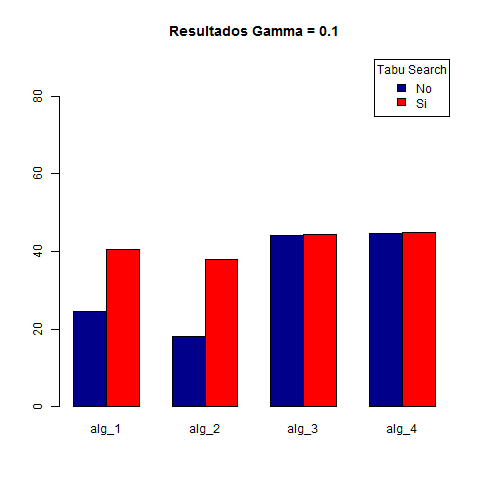
\includegraphics[width=0.25\textwidth]{img/gamma01.png}
	\caption{$\gamma$ = 0.1}
	\label{res:img-gamma01-papers}
\end{figure}

\begin{figure}[H]
	\centering
	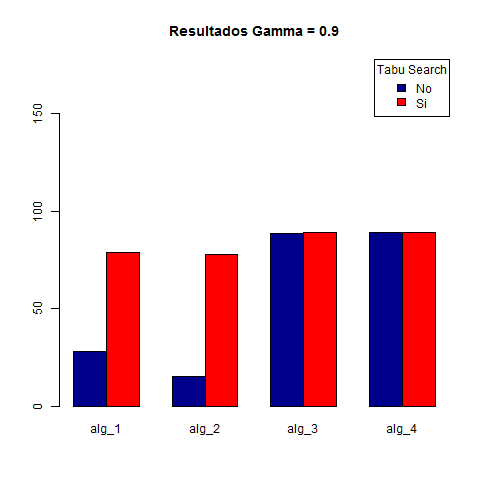
\includegraphics[width=0.25\textwidth]{img/gamma09.png}
	\caption{$\gamma$ = 0.9}
	\label{res:img-gamma09-papers}
\end{figure}
En la segunda búsqueda que se realizo se buscaron bundles de autores los cuáles no sean sean de la misma universidad de afiliación. Como similitud se cuenta con la función que compara el perfil de los autores y como complementaridad la universidad de pertenencia del autor.
\begin{figure}[H]
	\centering
	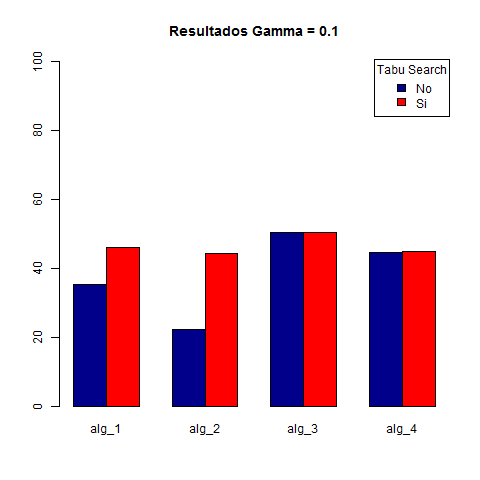
\includegraphics[width=0.25\textwidth]{img/gamma01-autores.png}
	\caption{$\gamma$ = 0.1}
	\label{res:img-gamma01-authors}
\end{figure}

\begin{figure}[H]
	\centering
	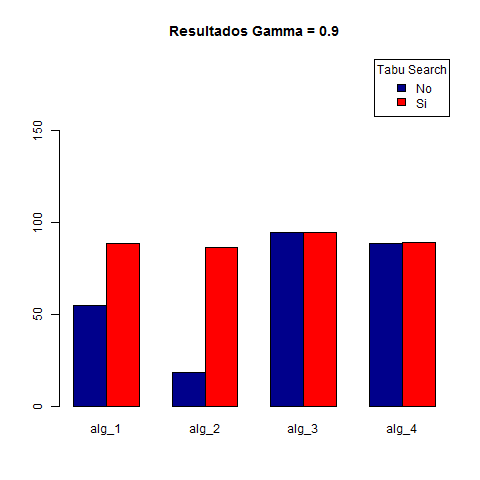
\includegraphics[width=0.25\textwidth]{img/gamma09-autores.png}
	\caption{$\gamma$ = 0.9}
	\label{res:img-gamma09-authors}
\end{figure}
\section{Conclusiones}
Como se ve en los gráficos del punto anterior el uso de la estrategía de búsqueda Tabú funcionó en todos los casos. Para el algoritmo BOBO la mejora fue significativamente mejor y no implicó ningún aumento considerable en el tiempo de ejecución, por lo cuál sin importar el algoritmo usado para generar la solución siempre se debe intentar mejorar mediante la búsqueda Tabú.\\
El fin de las búsquedas es poder ofrecerle al usuario una experiencia rápida como confiable que con éstos experimentos los algoritmos del estilo BOBO con el agregado de la una búsqueda Tabú al final mostro una relación muy favorable en cuanto a su timpo de ejecución y calidad de la solución (medida siempre con el valor de la función objetivo). Por esto mismo es conveniente trabajar en mejorar este tipo de huerísticas ya que son sencillas de implementar y agregan mucho overhead en la ejecución final de las búsquedas. En ~\ref{appendix-tables} pueden observarse los tiempos de las ejecuciones de los algoritmos y el valor final de la solución.
\section{Future work}
En un trabajo futuro se propone explorar las mismas búsquedas aquí presentadas pero tomando como ejemplo un paper que uno elija o un autor que le interese y generar bundles en el que cada uno de ellos este incluido el elemento específico que se usó para la búsqueda. Los elementos al ser tratados como un vector de $n$ posiciones, como se explicó en ~\ref{body-data-model}, podrían permitir más genericamente que se indiquen los porcentajes de cada uno de los temas involucrados que se quiera obtener un conjunto de soluciones.\\
Para un trabajo posterior se debe mejorar la implementación interna de los algoritmos para poder ejecutar en paralelelo partes de los algoritmos y depuración general de los mismos, ésto ayudado con un mejor diseño lógico de los datos pertenecientes al universo de búsqueda lograría una mejor performance general.\\
Se debe crear una nueva interfaz de usuario que sea amigable al interesado y muestre de forma prolija las soluciones obtenidas.\\
